\subsubsection{NXT-G}
Despite the NXT ship with the NXT-G programming language. NXT-G is a programming language based on LabView\cite{LabView}. The language uses a drag and drop block system, instead of writing code, illustrated in figure \ref{NXT-G}. This also provides a visual representation of the program.

\begin{figure}[H]
    \centering
    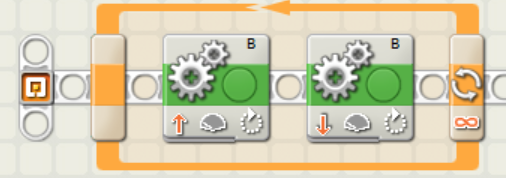
\includegraphics[width=0.7\textwidth]{Images/Software/Mindstorms/mindstorms_block.png}
    \caption{Ilustration of the drag and drop block system of NXT-G programming language}
    \label{NXT-G}
\end{figure}

This approach is easier to understand, but is limited when it comes to low level programming and when creating more complex programs. Luckily the NXT is a flexible platform, as it allows for custom firmware to be installed, which in turn allows for different programming languages to be used.
Some of these include RobotC\cite{RobotC}, leJOS\cite{leJOS} and nxtOSEK\cite{nxtOSEK}.

\subsubsection{RobotC}
This programming language is designed specifically for robot platforms. It is built on top of C, and is built with the primary purpose of being a educational platform. Noteworthy is that it is not free to use and requires a license.

\subsubsection{leJOS}
leJOS is a open-source firmware that includes the Java Virtual Machine\cite{Java}, and as such allows for writing Java programs. Originally written for LEGO RCX, a earlier version of the NXT, it has since been updated to run on the NXT.

leJOS has plugins for both Netbeans\cite{Netbeans} and Eclipse\cite{Eclipse} for making development more convenient.

\subsubsection{nxtOSEK} \label{nxtOSEK}
The firmware is a hybrid of leJOS and TOPPERS\cite{TOPPERS}. Using nxtOSEK it is possible to write C and C++ programs.

There are different ways to run nxtOSEK on a NXT. These approaches have different pros and cons, a listing of differences is shown in table \ref{firmCom}.
\begin{table}[H]
    \centering
    \label{firmware-comparison}
    \begin{tabular}{|l|l|l|l|}
    \hline
                                                                              & Memory                                                       & Programs & Interface \\ \hline
    Stock Firmware                                                                         & 64KB                                                         & Multiple & Stock     \\ \hline
    \begin{tabular}[c]{@{}l@{}}John Hansen's\\ Enhanced NXT Firmware\end{tabular} & 64KB                                                         & Multiple & Stock     \\ \hline
    NXTBios                                                                       & \begin{tabular}[c]{@{}l@{}}224KB ROM\\ 50KB RAM\end{tabular} & Single   & Barebone  \\ \hline
    \end{tabular}
    \caption{Comparison between firmware}
    \label{firmCom}
\end{table}

nxtOSEK supports scheduling using priority based scheduling\todo{Explain somewhere else and reference}. It uses alarms to define priorities and the execution rate.

\todo{Restructure all of this. Make a new subsection for scheduling: why it is needed (and why it's not needed in usual software projects). Reference the theory section for all kinds of different scheduling protocols and then present nxtOSEK and how it is a robust model that makes priority based scheduling simple. Decide that we are going to be using it.}
\info{To the todo above: I do not think that any mentioning of scheduling is needed as off yet, and that it will be sufficient that we haev already mentioned that we are dealing with real-time systems. Scheduling is an implicit component of real-time systems.}

\subsubsection{Choice of software}
We have chosen to go use the nxtOSEK because it does not cost us any money, it has the functionality that we need, and it allows for sufficiently low level programming languages, which is important when real-time systems are considered.